\documentclass[12pt]{beamer}
\usepackage{resume/dhuBeamer}

% 取消PDF压缩,加快速度,最终版本生成的时候需要把这句话注释掉
% \special{dvipdfmx:config z 0}


\title{东华大学 dhuBeamer 模板}
\subtitle{beamer 副标题}
\author[test]{测试}
\institute{测试学院}
\date{\today}


\begin{document}
\maketitle

\section{表格与图片}
\subsection{表格测试}

\begin{frame}
    \frametitle{字体大小设置}

    \begin{table}[H]
        \centering
        \scriptsize  % 设置 table 的字体大小
        \captionsetup{font = scriptsize}  % 设置 caption 的字体大小
        \caption{测试表格}
        \begin{tabular}{l|l|l}
            \toprule
            \textbf{参数}                & \textbf{搜索范围}       & \textbf{说明}            \\
            \midrule
            \texttt{n\_estimators}       & 750 -- 1250                              & 树的数量                  \\
            \texttt{learning\_rate}      & 0.01 -- 0.5 (对数搜索)                  & 学习率                   \\
            \texttt{num\_leaves}         & 50 -- 150                                & 控制树的复杂度            \\
            \texttt{max\_depth}          & 5 -- 15                                  & 树的最大深度              \\
            \texttt{min\_data\_in\_leaf} & 15 -- 30                                 & 每个叶子节点的最小样本数  \\
            \texttt{feature\_fraction}   & 0.5 -- 1.0                               & 每次迭代使用的特征比例    \\
            \texttt{bagging\_fraction}   & 0.7 -- 0.9                               & 每次迭代使用的样本比例    \\
            \texttt{bagging\_freq}       & 1 -- 5                                   & 执行 bagging 的频率       \\
            \texttt{min\_gain\_to\_split}& 0.01 -- 0.1                              & 分裂的最小增益            \\
            \bottomrule
        \end{tabular}
        \label{tab: hyperparameter_search_space}
    \end{table}

\end{frame}

\subsection{图片测试}
\begin{frame}
    \frametitle{图片测试}

    \begin{figure}[H] % 图片位于文字下方
        \centering % 居中
        % 设置图片占页面宽度的比例(默认0.8)
        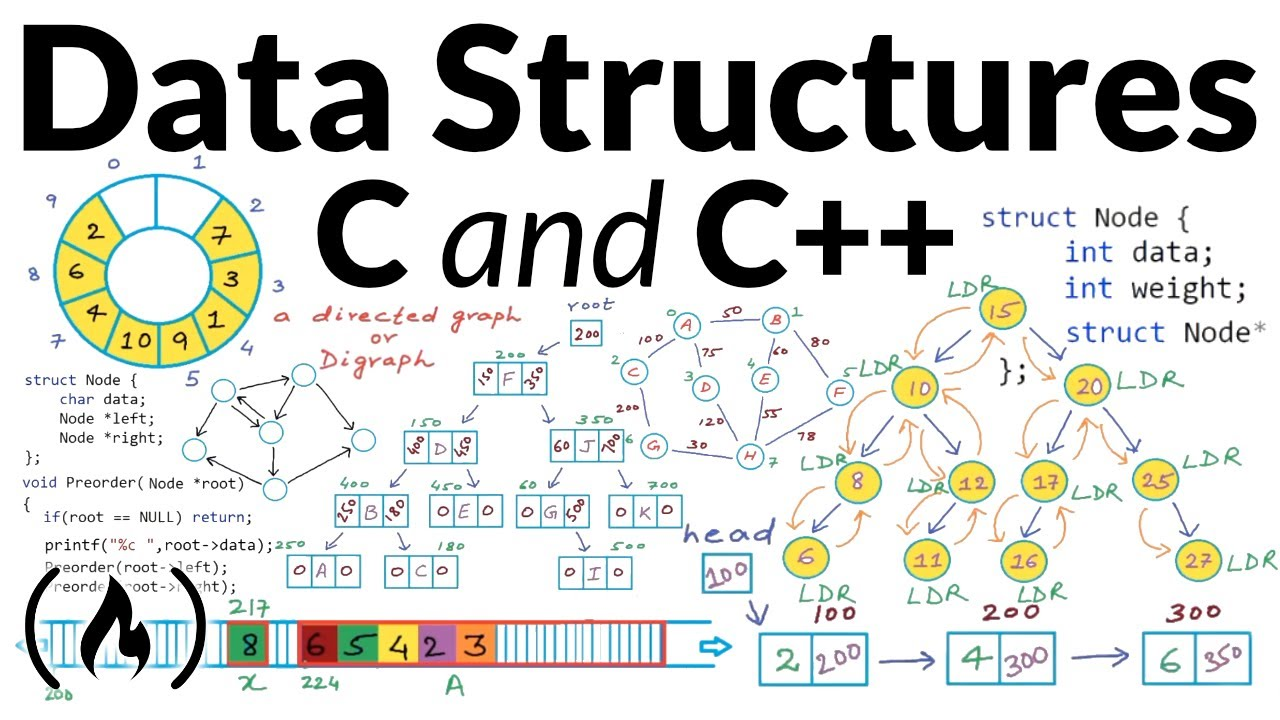
\includegraphics[width=0.6\textwidth]{assets/dataStructures.jpg}
        \captionsetup{font = scriptsize}  % 设置 caption 的字体大小
        \caption{图片标题} % 图例,按章节编号
        \label{fig: 数据结构2} % 图片索引
    \end{figure}
\end{frame}

\makebottom{感谢使用 dhuBeamer 模板}
\end{document}